% ai-phishing-detection-dissertation/report/sections/4-results/random-forest-model-performance/performance-on-internal-test-set.tex

\subsubsection*{Performance on internal test set}
The Random Forest was trained upon 29,280 samples from the primary training corpus, consisting of the combined dataset comprising of Enron (ham) and CEAS 2008 (phishing). The initial training pass was achieved in \textbf{24.82 seconds} and achieved a training accuracy of \textbf{0.9904}.\newline

\noindent Hyperparemter tuning was performed with "\texttt{GridSearchCV}" using a 3-fold cross-validation, to optimise parameters for this model, taking \textbf{22 minutes} for optimisation.

\begin{table}[h]
\centering
\begin{tabularx}{\textwidth}{|X|X|}
\hline
\textbf{Parameter} & \textbf{Optimised value} \\
\hline
\texttt{criterion} & \texttt{entropy} \\
\hline
\texttt{max\_depth} & \texttt{None} \\
\hline
\texttt{min\_samples\_leaf} & \texttt{2} \\
\hline
\texttt{min\_samples\_split} & \texttt{5} \\
\hline
\texttt{n\_estimators} & \texttt{100} \\
\hline
\end{tabularx}
\caption{Optimised Random Forest hyperparameters}
\end{table}

\noindent The tuned model achieved an accuracy of \textbf{0.9833}, and a weighted F1-score of \textbf{0.9833} on the reserved validation set. Per-class performance is detailed in the below table.

\begin{table}[h]
\centering
\begin{tabularx}{\textwidth}{|X|X|}
\hline
\textbf{Metric} & \textbf{Value} \\
\hline
Precision (Ham) & \texttt{0.98} \\
\hline
Recall (Ham) & \texttt{0.98} \\
\hline
F1-Score (Ham) & \texttt{0.98} \\
\hline
Precision (Phish) & \texttt{0.98} \\
\hline
Recall (Phish) & \texttt{0.99} \\
\hline
F1-Score (Phish) & \texttt{0.98} \\
\hline
Accuracy & \texttt{0.9833} \\
\hline
Weighted F1 & \texttt{0.9833} \\
\hline
\end{tabularx}
\caption{Classification report metrics (Support: Ham = 3000, Phish = 3274)}
\end{table}

\noindent The final tuned Random Forest model was evaluated on the internal test set of 6,275 samples from the Enron and CEAS split not used during training or even hyperparameter tuning. The performance metrics on this internal test set are presented in the following table, along with the relevant confusion matrix.

\begin{table}[h]
\centering
\begin{tabularx}{\textwidth}{|X|X|}
\hline
\textbf{Metric} & \textbf{Value} \\
\hline
Accuracy & \texttt{0.9815} \\
\hline
Precision (Phishing) & \texttt{0.9782} \\
\hline
Recall (Phishing) & \texttt{0.9866} \\
\hline
F1-Score (Phishing) & \texttt{0.9824} \\
\hline
ROC AUC Score & \texttt{0.9988} \\
\hline
\end{tabularx}
\caption{Random Forest performance on internal yest set}
\end{table}

\begin{figure}[H]
  \begin{center}
    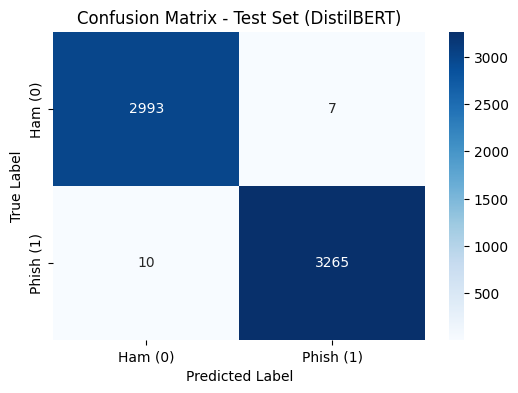
\includegraphics[scale=0.9]{confusion-matrices/random-forest/internal-test-set.png}
    \caption{Confusion matrix illustrating the performance of the tuned Random Forest model on the internal test set, showing true positives, true negatives, false positives, and false negatives}
  \end{center}
\end{figure}

\noindent The classification report for the internal test set is presented in the below table.

\begin{table}[h]
\centering
\begin{tabularx}{\textwidth}{|X|X|X|X|X|}
\hline
\textbf{Class} & \textbf{Precision} & \textbf{Recall} & \textbf{F1-Score} & \textbf{Support} \\
\hline
Ham (0) & \texttt{0.99} & \texttt{0.98} & \texttt{0.98} & \texttt{3000} \\
\hline
Phish (1) & \texttt{0.98} & \texttt{0.99} & \texttt{0.98} & \texttt{3275} \\
\hline
Accuracy  &  &  & \texttt{0.98} & \texttt{6275} \\
\hline
Macro Avg & \texttt{0.98} & \texttt{0.98} & \texttt{0.98} & \texttt{6275} \\
\hline
Weighted Avg & \texttt{0.98} & \texttt{0.98} & \texttt{0.98} & \texttt{6275} \\
\hline
\end{tabularx}
\caption{Random Forest classification report on internal test set}
\end{table}

\noindent The results show that the Random Forest model has a strong performance on the internal test set, proved by the high precision and recall values, particularly for the phishing class.
